\documentclass[12pt]{beamer}

\usepackage{color}
\usepackage[normalem]{ulem}
\usepackage[font=scriptsize]{caption}

% Esto es para que el LaTeX sepa que el texto est� en espa�ol:
\usepackage[spanish]{babel}

% Include figure files.
\usepackage{graphicx}

% Author, Title, etc.

\title[Bases de Datos Espacio-Temporales] 
{%
  Bases de Datos Espacio-Temporales%
}

\author[Del Piano]
{
  Nicol\'as Del Piano
}

\date
{
Bases de Datos Avanzadas
}

\mode<presentation>{
\usetheme{boxes}
\useinnertheme{}
\usecolortheme{whale}
}\setbeamercolor{structure}{fg=blue!50!black!70}
\setbeamertemplate{footline}[frame number]
\setbeamerfont{page number in head/foot}{size=\normalsize}

\newenvironment{variableblock}[3]{%
  \setbeamercolor{block body}{#2}
  \setbeamercolor{block title}{#3}
  \begin{block}{#1}}{\end{block}}

\setbeamercolor{block title}{bg=red!60,fg=black}
%\setbeamertemplate{blocks}[rounded][shadow=true] 
\setbeamercolor{postit}{bg=yellow!50!white}
\setbeamercolor{bluelick}{bg=blue!50!white}

\begin{document}
\frame{\titlepage}
\begin{frame}
\frametitle{Recorrido}
\begin{itemize}
\item Bases de Datos Espacio-Temporales
\begin{enumerate}
\item Definici\'on
\item Importancia
\item Apliaciones
\item Requerimientos
\item Modelo Espacio-Temporal
\end{enumerate}
\item Lenguajes de Consulta
\begin{enumerate}
\item Lenguaje de G\"uting
\item Lenguaje SQL$^{ST}$
\end{enumerate}
\item Estado del Arte
\end{itemize}
\end{frame}

\begin{frame}
\frametitle{Bases de Datos Espacio-Temporales}
El objetivo es extender los modelos de informaci\'on espacial para inclu\'ir tiempo y describir de forma m\'as din\'amica la realidad que se quiere representar. 
\end{frame}

\begin{frame}
\frametitle{Bases de Datos Espacio-Temporales}
Se han convertido en un t\'opico muy imporante en estos \'ultimos a\~nos, ya que muchas de las aplicaciones como los Sistemas de Informaci\'on Geogr\'afica y los sistemas de localizaci\'on necesitan almacenar datos espaciales con caracter\'isticas temporales.
\end{frame}

\begin{frame}
\frametitle{Bases de Datos Espacio-Temporales}
\begin{variableblock}{STDB}{bg=blue!50!white!70,fg=white}{bg=blue!50!black!70,fg=white}
\textit{Un STDBMS es un DBMS cuyo aporte esencial es el manejo de datos espaciales a trav\'es del tiempo.}
\end{variableblock}
\ \\
\begin{figure}[fig1]
\centering
\begin{minipage}{.4\textwidth}
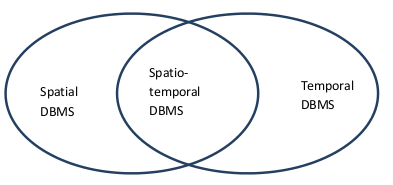
\includegraphics[width=\textwidth]{images/figure1.png}
\caption{Una idea de la relaci\'on entre la informaci\'on espacial, temporal y espacio-temporal.}
\end{minipage}
\end{figure}
\end{frame}

\begin{frame}
\frametitle{Importancia}
Muchas de las aplicaciones de bases de datos tratan el fen\'omeno espacio-temporal, y durante esta \'ultima d\'ecada muchos grupos de investigaci\'on han investigado sobre la predicci\'on del clima, prevenci\'on del atascamiento del tr\'afico, servicios de localizaci\'on, movimiento de objetos, etc\'etera.
\end{frame}

\begin{frame}
\frametitle{Importancia}
Proveer un modelo DBMS para dar soporte al fen\'omeno espacio-temporal se convirti\'o en un aspecto importante.\\
\ \\
S\'olo muy pocos STDBMS existen para satistfacer los tipos de datos y operaciones espacio-temporales.
\end{frame}

\begin{frame}
\frametitle{Aplicaciones}
El modelo espacio-temporal abarca aplicaciones:
\begin{itemize}
\item Demogr\'aficas
\item Ecol\'ogicas
\item Marketing
\item Fen\'omenos naturales
\item Militares
\item Urban\'isticas
\end{itemize}
\end{frame}


\begin{frame}
\frametitle{Requerimientos}
\begin{itemize}
\item Representaci\'on eficiente del espacio y el tiempo.
\begin{itemize}
\item Heredado de los modelos espaciales y temporales.
\end{itemize}
\item Modelos de datos
\begin{itemize}
\item Representa la evoluci\'on temporal de los objetos espaciales, a trav\'es de nuevos tipos de datos, las operaciones y relaciones entre ellos.
\end{itemize}
\item Lenguajes de consulta

\end{itemize}
\end{frame}

\begin{frame}
\frametitle{STDB}
Una base de datos espacio-temporal necesita proveer un soporte DBMS para mover objetos que cambian cont\'inuamente de forma y posici\'on.
\begin{figure}
\centering
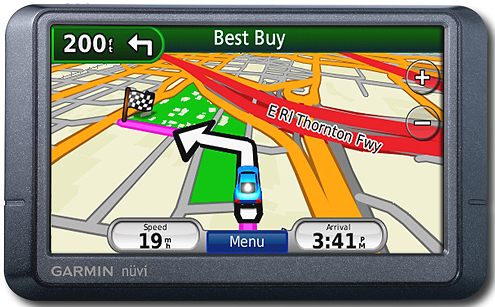
\includegraphics[scale=0.3]{images/figure2.png}
\caption{Los GPS han introducido una fuerte demanda para implementar STDBMS eficientes.}
\end{figure}
\end{frame}

\begin{frame}
\frametitle{Modelo Espacio-Temporal}
Los tipos de datos espacio-temporales permiten al usuario describir un comportamiento din\'amico de objetos espaciales a trav\'es del tiempo.\\
\ \\
El objeto espacial se mueve $\Rightarrow$ los llamamos \textit{moving objects}.\\
\ \\
De la misma forma que los objetos espaciales, los espacio-temporales son a\~nadidos como atributos de tipo en un modelo de datos de un DBMS.

\end{frame}

\begin{frame}
\frametitle{Tipos de Datos Espacio-Temporales}
MPOINT (moving point), MLINE (moving line) y MREGION (moving region).\\
\ \\
Conceptualmente:\\
MPOINT es una funci\'on $f : time \rightarrow point$\\
MLINE es una funci\'on $f : time \rightarrow line$\\
MREGION es una funci\'on $f : time \rightarrow region$\\
\begin{figure}
\centering
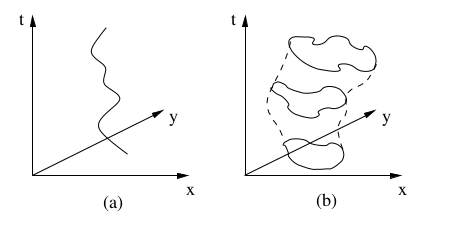
\includegraphics[scale=0.4]{images/figure22.png}
\caption{Ejemplos de un objeto \textit{moving point} (a) y un objeto \textit{moving region} (b).}
\end{figure}
\end{frame}

\begin{frame}
\frametitle{Operaciones y Predicados}
Algunas de las operaciones que un modelo espacio-temporal debe ofrecer (adem\'as de las espaciales y temporales):\\
\ \\
$deftime: mpoint \rightarrow periods$\\
$Disjoint: mpoint \times mregion \rightarrow bool$\\
$distance: mpoint \times mpoint \rightarrow mreal$\\
$Inside: mpoint \times mregion \rightarrow bool$\\
$intersection: mpoint \times mregion \rightarrow mpoint$\\
$meet: point \times region \rightarrow bool$\\
$min: mreal \rightarrow real$\\
$trajectory: mpoint \rightarrow line$\\
\end{frame}

\begin{frame}
\begin{center}
\textbf{LENGUAJES DE CONSULTA ESPACIO-TEMPORALES}
\end{center}
\end{frame}

\begin{frame}
\frametitle{Lenguajes de Consulta Espacio-Temporales}
Se han propuesto diversos lenguajes de consulta para este tipo de base de datos, como por ejemplo, SQL$^{ST}$ (Chen y Zaniolo, 2000), G\"uting (G\"uting y Schneider, 2005), el de Chomicki (Chomicki y Revesz, 1999) y STQL (Erwig y Schneider, 2002) entre otros.\\
\ \\
En esta clase veremos y compararemos los dos primeros.
\end{frame}

\begin{frame}
\frametitle{Caso de estudio}
\textbf{Escenario:} incendio forestal (G\"uting et \'al., 2000; Chen y Zaniolo, 2000).\\
\ \\
Se maneja informaci\'on sobre bosques, incendios y bomberos.
\end{frame}

\begin{frame}
\frametitle{Lenguajes de Consulta: G\"uting}
En G\"uting y Schneider (2005) se propone un lenguaje de consulta para el manejo de objetos m\'oviles (se soportan cambios cont\'inuos de las geometr\'ias, ya sea en forma y posici\'on).\\
\ \\
Se proponen tipos de datos m\'oviles como MBOOL, MINTEGER, MPOINT, MLINE y MREGION, que combinan los tipos de datos primitivos y los espaciales con informaci\'on temporal.\\
\ \\
Lenguaje de tipo SQL.
\end{frame}

\begin{frame}
\frametitle{Lenguajes de Consulta: G\"uting}

\begin{variableblock}
{Creaci\'on de las tablas}{bg=blue!50!white!70,fg=white}{bg=blue!50!black!70,fg=white}
\texttt{Bosque (nombre: STRING, territorio: REGION)\\
Incendio (nombre: STRING, extensi\'on: MREGION)\\
Bombero (nombre: STRING, ubicaci\'on: MPOINT)
}
\end{variableblock}

\begin{figure}
\centering
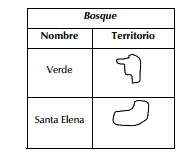
\includegraphics[scale=0.4]{images/tabosque1.png}
\caption{Tabla bosque para el lenguaje de G\"uting.}
\end{figure}
\end{frame}

\begin{frame}
\frametitle{Lenguajes de Consulta: G\"uting}

\begin{figure}
\centering
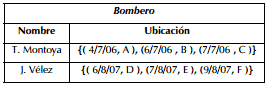
\includegraphics[scale=0.4]{images/tabomberoguting.png}
\caption{Tabla bombero para el lenguaje de G\"uting.}
\end{figure}

\begin{figure}
\centering
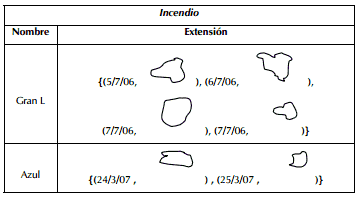
\includegraphics[scale=0.4]{images/tabincendioguting.png}
\caption{Tabla incendio para el lenguaje de G\"uting.}
\end{figure}
\end{frame}

\begin{frame}
\frametitle{Lenguajes de Consulta: SQL$^{ST}$}
SQL$^{ST}$ (Chen y Zaniolo, 2000) es una extensi\'on minimalista del SQL est\'andar, ya que preserva su estructura y s\'olo a\~nade tipos de datos temporales (DAY), espaciales (POINT, LINE y REGION) y operadores (\'AREA, OVERLAP, MOVING\_DISTANCE).\\
\ \\
El tiempo se representa en forma discreta, as\'i los cambios en las geometr\'ias son discretos.

\end{frame}

\begin{frame}
\frametitle{Lenguajes de Consulta: SQL$^{ST}$}

\begin{variableblock}
{Creaci\'on de las tablas}{bg=blue!50!white!70,fg=white}{bg=blue!50!black!70,fg=white}
\texttt{CREATE TABLE bosque (nombre CHAR(30), territorio REGION)\\
CREATE TABLE incendio (nombre CHAR(30), extensi\'on REGION, d\'ia DAY)\\
CREATE TABLE bombero (nombre CHAR(30), ubicaci\'on POINT, d\'ia DAY)
}
\end{variableblock}

\begin{figure}
\centering
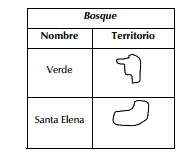
\includegraphics[scale=0.4]{images/tabosque1.png}
\caption{Tabla bosque para el lenguaje SQL$^{ST}$.}
\end{figure}
\end{frame}

\begin{frame}
\frametitle{Lenguajes de Consulta: SQL$^{ST}$}
\begin{figure}
\centering
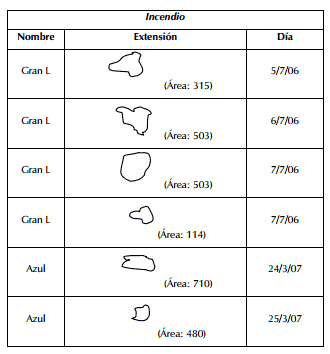
\includegraphics[scale=0.4]{images/tablaincendiosqlts.png}
\caption{Tabla incendio para el lenguaje SQL$^{ST}$.}
\end{figure}
\end{frame}

\begin{frame}
\frametitle{Lenguajes de Consulta: SQL$^{ST}$}
\begin{figure}
\centering
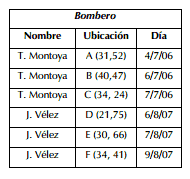
\includegraphics[scale=0.4]{images/tablabomberosqlts.png}
\caption{Tabla bombero para el lenguaje SQL$^{ST}$.}
\end{figure}
\end{frame}

\begin{frame}
\frametitle{Ejemplos de consultas}
?`C\'uando y d\'onde alcanz\'o el incendio "Gran L" su m\'axima extensi\'on?
\begin{variableblock}
{Consulta: G\"uting}{bg=blue!50!white!70,fg=white}{bg=blue!50!black!70,fg=white}
\texttt{LET GranL = ELEMENT(SELECT extensi\'on\\
\ \ \ \ FROM incendio\\
\ \ \ \ WHERE nombre = "Gran L");\\
LET max\_area = INITIAL(ATMAX(AREA(GranL)));\\
ATINSTANT(GranL, INST(max\_area));\\
VAL(max\_area);}
\end{variableblock}

%\begin{tabular}{c c}
\begin{figure}
\centering
\begin{tabular}{c c}
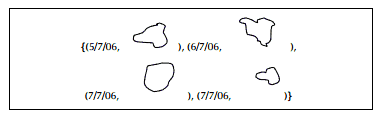
\includegraphics[scale=0.4]{images/consultaGranL1.png}
%\caption{Este es el resultado de GranL.}
%\end{figure}
&
%\begin{figure}
%\centering
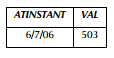
\includegraphics[scale=0.4]{images/consultaGranL2.png}
\end{tabular}
\caption{La primer figura nos muestra el resultado de GranL. En la segunda, el resultado de la consulta.}
\end{figure}

%\end{tabular}

\end{frame}


\begin{frame}
\frametitle{Ejemplos de consultas}
?`C\'uando y d\'onde alcanz\'o el incendio "Gran L" su m\'axima extensi\'on?
\begin{variableblock}
{Consulta: SQL$^{ST}$}{bg=blue!50!white!70,fg=white}{bg=blue!50!black!70,fg=white}
\texttt{SELECT d\'ia, extensi\'on, AREA(extensi\'on)\\
FROM incendio\\
WHERE nombre = "Gran L" AND AREA(extensi\'on) =\\
\ \ \ \ SELECT MAX(AREA(extensi\'on))\\
\ \ \ \ \ \ FROM incendio\\
\ \ \ \ \ \ WHERE nombre = "Gran L");\\}
\end{variableblock}

%\begin{tabular}{c c}
\begin{figure}
\centering

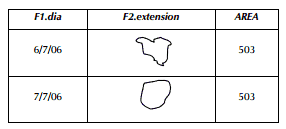
\includegraphics[scale=0.4]{images/resultadosqlst1.png}
\caption{Este es el resultado de la consulta.}
%\end{figure}
\end{figure}

%\end{tabular}

\end{frame}

\begin{frame}
\frametitle{Ejemplos de consultas}
?`C\'uando y d\'onde se expandieron los incendios m\'as de 500 km$^{2}$?
\begin{variableblock}
{Consulta: G\"uting}{bg=blue!50!white!70,fg=white}{bg=blue!50!black!70,fg=white}
\texttt{LET reg\_grande = SELECT a\_grande AS extensi\'on\\
WHEN[FUN(r:region) AREA(r) $>$ 500]\\
\ \ \ \ FROM incendio;\\
SELECT * FROM reg\_grande\\
WHERE NOT(ISEMPTY(DEFTIME(a\_grande)));\\}
\end{variableblock}

%\begin{tabular}{c c}
\begin{figure}
\centering
\begin{tabular}{c c}
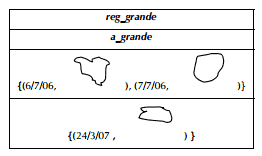
\includegraphics[scale=0.4]{images/reg_grande1.png}
%\caption{Este es el resultado de GranL.}
%\end{figure}
&
%\begin{figure}
%\centering
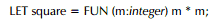
\includegraphics[scale=0.4]{images/square.png}
\end{tabular}
\caption{La primer figura nos muestra el valor de reg\_grande. En la segunda, la cl\'ausula FUN.}
\end{figure}

%\end{tabular}

\end{frame}

\begin{frame}
\frametitle{Ejemplos de consultas}
?`C\'uando y d\'onde se expandieron los incendios m\'as de 500 km$^{2}$?
\begin{variableblock}
{Consulta: SQL$^{ST}$}{bg=blue!50!white!70,fg=white}{bg=blue!50!black!70,fg=white}
\texttt{SELECT d\'ia, extensi\'on\\
FROM incendio\\
WHERE AREA(extensi\'on) > 500;\\}
\end{variableblock}

%\begin{tabular}{c c}
\begin{figure}
\centering
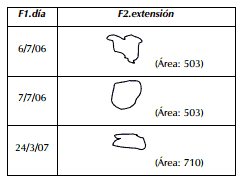
\includegraphics[scale=0.4]{images/consulta2sqlst.png}
%\caption{Este es el resultado de GranL.}
%\end{figure}

%\begin{figure}
%\centering
\caption{El resultado de la consulta en SQL$^{ST}$.}
\end{figure}

%\end{tabular}

\end{frame}

\begin{frame}
\frametitle{Ejemplos de consulta}
?`Cu\'anto tiempo estuvo el bombero \textit{T. Montoya} dentro de \textit{Gran L} y cu\'anta distancia recorri\'o dentro?
\begin{figure}
\centering
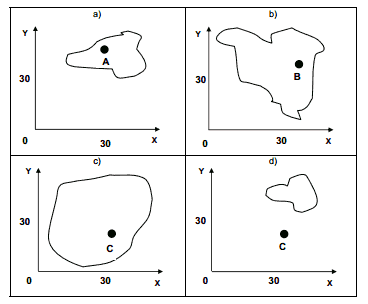
\includegraphics[scale=0.4]{images/movbombero.png}
\caption{Ubicaci\'on del bombero \textit{T. Montoya} dentro de \textit{Gran L}: a) punto A y regi\'on 315 km$^{2}$ el 5/7/06, b) punto B y regi\'on de 503 km$^{2}$ el 6/7/06, c) punto C y regi\'on de 503 km$^{2}$ el 7/7/06 y d) punto D y regi\'on de 114 km$^{2}$ el 7/7/06.}
\end{figure}
\end{frame}


\begin{frame}
\frametitle{Ejemplos de consultas}
?`Cu\'anto tiempo estuvo el bombero \textit{T. Montoya} dentro de \textit{Gran L} y cu\'anta distancia recorri\'o dentro?
\begin{variableblock}
{Consulta: SQL$^{ST}$}{bg=blue!50!white!70,fg=white}{bg=blue!50!black!70,fg=white}
\texttt{SELECT DURATION(bombero.d\'ia),\\
\ \ \ \ MOVING\_DISTANCE(bombero.ubicaci\'on,\\
\ \ \ \ \ \ bombero.d\'ia)\\
FROM incendio, bombero\\
WHERE incendio.d\'ia = bombero.d\'ia AND\\
\ \ \ incendio.nombre = "Gran L" AND\\
\ \ \ bombero.nombre = "T. Montoya" AND\\
\ \ \ INSIDE (bombero.ubicacion, incendio.extensi\'on)}
\end{variableblock}

\end{frame}

\begin{frame}
\frametitle{Ejemplos de consulta}
?`Cu\'anto tiempo estuvo el bombero \textit{T. Montoya} dentro de \textit{Gran L} y cu\'anta distancia recorri\'o dentro?
\begin{figure}
\centering
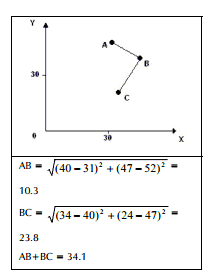
\includegraphics[scale=0.4]{images/funcionmovingdistance.png}
\caption{Ejemplo de la funci\'on MOVING\_DISTANCE.}
\end{figure}
\end{frame}

\begin{frame}
\frametitle{Ejemplos de consulta}
?`Cu\'anto tiempo estuvo el bombero \textit{T. Montoya} dentro de \textit{Gran L} y cu\'anta distancia recorri\'o dentro?
%\begin{tabular}{c c}
\begin{figure}
\centering
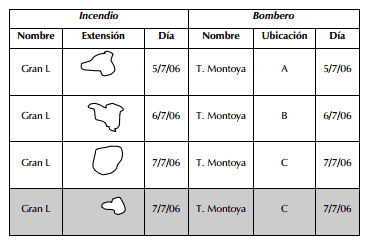
\includegraphics[scale=0.4]{images/consulta3sqlst.png}
%\caption{Este es el resultado de GranL.}
%\end{figure}

%\begin{figure}
%\centering
\caption{Resultado parcial de la consulta en SQL$^{ST}$.}
\end{figure}

\begin{figure}
\centering
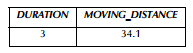
\includegraphics[scale=0.4]{images/consulta3sqlst2.png}
\caption{Resultado de la consulta en SQL$^{ST}$.}
\end{figure}

%\end{tabular}
\end{frame}

\begin{frame}
\frametitle{Ejemplos de consulta}
?`Cu\'anto tiempo estuvo el bombero \textit{T. Montoya} dentro de \textit{Gran L} y cu\'anta distancia recorri\'o dentro?
\begin{variableblock}
{Consulta: G\"uting}{bg=blue!50!white!70,fg=white}{bg=blue!50!black!70,fg=white}
\texttt{SELECT tiempo AS\\
DURATION (DEFTIME (INTERSECTION (ubicaci\'on, GranL))),\\
\ \ \ \ distancia AS LENGTH(TRAJECTORY(INTERSECTION(ubicaci\'on,GranL)))\\
FROM bombero\\
WHERE nombre = "T. Montoya";}
\end{variableblock}
\begin{figure}
\centering
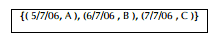
\includegraphics[scale=0.4]{images/gutinguin.png}
\caption{MPOINT resultante de INTERSECTION(ubicaci\'on, GranL).}
\end{figure}
\end{frame}

\begin{frame}
\begin{center}
\textbf{ESTADO DEL ARTE}
\end{center}
\end{frame}

\begin{frame}
\frametitle{Actualidad de las STDB}
Las STDB tratan con aplicaciones donde los tipos de datos son caracterizados por informaci\'on espacial y temporal.\\
\ \\
La implementaci\'on e investigaci\'on en este \'area ha empezado d\'ecadas atr\'a, cuando el manejo y manipulaci\'on de datos relacionada a los aspectos temporales y espaciales se hizo indispensable.
\ \\
Sin embargo, no es una tarea sencilla dado la complejidad de las estructuras de datos junto con la representaci\'on y manipulaci\'on de esa informaci\'on involucrada.
\end{frame}

\begin{frame}
\frametitle{Actualidad Espacio-Temporal}
Una alternativa para lidiar con la informaci\'on espacio-temporal, es constru\'ir un DBMS especializado para dar un soporte eficiente a los tipos de datos y consultas (\textbf{CONCERT} (Relly et al. 1997) y \textbf{SECONDO} (Dieker y G\"uting 2000)).\\
\ \\
Cuando no sea posible usar un DBMS especializado, otra alternativa ser\'ia extender un DBMS (orientado a objetos o relacional), ya sea open source o comercial, para la manipulaci\'on y almacenamiento de objetos espacio-temporales.
\end{frame}

\begin{frame}
\frametitle{Actualidad Espacio-Temporal}
Aunque los DBMS tienen capacidad de extenderse y mecanismos para soportar estas necesidades espacio-temporales, no existe un DBMS open source con una extensi\'on espacio-temporal.\\
\ \\
Otra alternativa es crear una arquitectura por capas sobre una DBMS ya existente.\\
\ \\
\textit{Oracle} brinda soporte espacio-temporal con las \textit{versioned tables} de su Workspace Manager, pero es comercial.
\end{frame}

\begin{frame}
\frametitle{TerraLib}
Es una librer\'ia GIS open source que extiende el modelo relacional de un DBMS para el manejo del modelo de datos espacio temporal.\\
\ \\
\begin{figure}
\begin{center}

\includegraphics[scale=0.4]{images/terralib.png}
\caption{www.terralib.org}
\end{center}
\end{figure}
\ \\
Soporta diferentes DBMS, incluyendo Oracle, PostgreSQL y MySQL. Se programa en C++.\\
\ \\
Tiene su centro de desarrollo en Brasil y se distribuye bajo la licencia LGPL.
\end{frame}

\begin{frame}
\frametitle{TerraLib}
Existen varias aplicaciones asociadas para facilitar la visualizaci\'on de consultas y el manejo del usuario.\\
\ \\
\begin{figure}
\centering
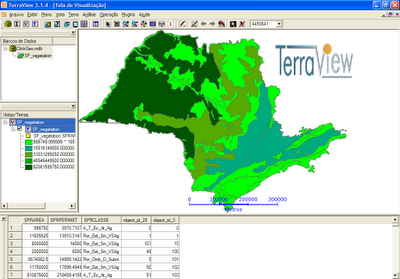
\includegraphics[scale=0.4]{images/terraview.png}
\caption{TerraView, un entorno gr\'afico para utilizar TerraLib.}
\end{figure}
\end{frame}

\begin{frame}
\frametitle{Problema}
Existen numerosas bases de datos relacionales con extensiones espaciales y temporales, pero las bases de datos espacio-temporales no est\'an basadas en el modelo relacional por razones pr\'acticas.\\
\ \\
Hasta ahora no hay RDBMS con extensiones espacio-temporales incorporadas.\\
\ \\
TerraLib es como un medio externo que las utiliza para brindar estas herramientas.
\end{frame}

\begin{frame}
\frametitle{The Google Approach}
Ya conocemos el inmenso trabajo de esta compan\'ia en los aspectos espacio-temporales.\\
\ \\
Entonces, ?` c\'omo lidia Google este tipo de problemas? 
\end{frame}

\begin{frame}
\frametitle{KML}
Keyhole Markup Language es una notaci\'on XML para representar datos geogr\'aficos en 3 dimensiones.\\
\ \\
Permite describir y almacenar informaci\'on geogr\'afica as\'i como tambi\'en incorporar temporal.\\
\ \\
KML es un est\'andar abierto y de su mantenimiento se encarga el Open Geospatial Consortium. Fue desarrollado para Google Earth y Google Maps.
\end{frame}

\begin{frame}
\frametitle{Google Earth}
En Google Earth 5 se implement\'o la visualizaci\'on de im\'agenes hist\'oricas. Es decir, podemos ver c\'omo se ha ido construyendo el edificio al lado de casa, o c\'omo era el entorno de nuestro pueblo a\~nos atr\'as.\\
\ \\
\begin{figure}
\centering
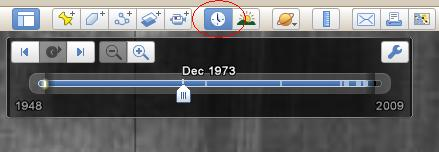
\includegraphics[scale=0.4]{images/earth.jpg}
\caption{Google Earth 5 y su herramienta hist\'orica.}
\end{figure}
\end{frame}

\begin{frame}
\frametitle{KML: Ejemplo}

\begin{variableblock}{El tiempo con vistas abstractas (fragmento).}{bg=blue!50!white!70,fg=white}{bg=blue!50!black!70,fg=white}
\texttt{$<$Placemark$>$\\
\ \ $<$name$>$Palace of Fine Arts in 2002$<$/name$>$\\
\ \ $<$Camera$>$\\
\ \ \ $<$gx:TimeStamp$>$\\
\ \ \ \ \ $<$when$>$2002-07-09T190:00:00-08:00$<$/when$>$ \\
\ \ \ $<$/gx:TimeStamp$>$\\}
\end{variableblock}

\end{frame}

\begin{frame}
\frametitle{KML: Ejemplo}
Y tambi\'en describir objetos espaciales:\\
\ \\
\begin{variableblock}{Descripci\'on en el mapa de New York City}{bg=blue!50!white!70,fg=white}{bg=blue!50!black!70,fg=white}
\texttt{$<$?xml version="1.0"$>$\\
$<$Document$>$\\
$<$Placemark$>$\\
\  $<$name$>$New York City$<$/name$>$\\
\ \ $<$description$>$New York City$<$/description$>$\\
\ \ $<$Point$>$\\
\ \ \ \ $<$coordinates$>$-74.0063,40.7141,0$<$/coordinates$>$\\
\ \ $<$/Point$>$\\
$<$/Placemark$>$\\
$<$/Document$>$\\
$<$/kml$>$}
\end{variableblock}
\end{frame}
\begin{frame}
\frametitle{Otros formatos de datos espacio-temporales}
\begin{itemize}
\item XML en s\'i
\item GML
\item NetCDF
\begin{itemize}
\item Es un formato de archivo, dise\~nado para leer y escribir eficientemente matrices de datos.
\end{itemize}
\end{itemize}
\end{frame}

%\begin{variableblock}{ROSE (RObust Spatial Extension, G\"uting \& Schneider)}{bg=blue!50!white!70,fg=white}{bg=blue!50!black!70,fg=white}
%\textit{Es un \'algebra espacial con tipos de datos espaciales basados en el modelo Realm (esto es, objetos compuestos por elementos realm)}
%\end{variableblock}

\begin{frame}
\frametitle{Bibliograf\'ia}
\begin{itemize}
\item R. H. G\"uting and M. Schneider. Moving Objects Databases.
\item Spatial and Spatio-Temporal Data Models and Languages, Markus Schneider.
\item Claudia Deco y Cristina Bender. T\'opicos Avanzados de Bases de Datos.
\item Cyndy Xinmin Chen and Carlo Zaniolo. SQL$^{ST}$: A Spatio-Temporal Data Model and Query Language.
\end{itemize}
\end{frame}

\end{document}